\section{Review Methodology}

Pilot study:\\
\\
Firstly, we wanted to work in security and we chose the more specific topic "Contract signing". When searching on IEEE Xplore, we found many related articles : 336 results, which was too much and would have required a lot more time. We narrowed down the research subject by adding the "optimistic" and "abuse-free" keywords and got more relevant publications. As we found only 4 papers on IEEE Xplore, we chose Scopus as our reference database and got 14 results. Using these research questions, we now want to move forward in the SLR in addressing gaps with contract signing for any number of signers using RSA.\\
\\
DataBase Selection: 
\\
We selected Scopus and IEEE to carry out our database search as they are well known in our domain of interest and known to give out quality results. Scopus database is not only elaborate but also has subscriptions to patent databases which implies that a wide coverage of search results. IEEE is the second database we selected for our search as IEEE also has a broad coverage of articles and known for top notch contributions from its wide member network. We want to limit our database search only to reputed databases because data from the articles is very important to our research of interest and that should not be compromised.   
\\
Search Strings:\\
\\
Security is the domain initially chosen, with more specific application : "Contract signing". As the topic is huge and requires much time, we narrow it down by adding the keywords "Optimistic" and "Abuse-Free" as we are more interested with these protocols. A basic search is performed, and papers found are analysed and synthesised in table \ref{table:results}. After the initial search with the string “Contract Signing”, we updated it to ( TITLE-ABS-KEY ( optimistic )  AND  TITLE-ABS-KEY ( contract  signing ) ) which returned 63 results, we then appended keyword “Abuse-Free” and updated our search string to ( TITLE-ABS-KEY ( optimistic )  AND  TITLE-ABS-KEY ( contract  signing )  AND  TITLE-ABS-KEY ( abuse-free ) ), we then applied our Inclusion and Exclusion criteria and string is updated to ( TITLE-ABS-KEY ( optimistic )  AND  TITLE-ABS-KEY ( contract  signing )  AND  TITLE-ABS-KEY ( abuse-free ) )  AND  ( LIMIT-TO ( DOCTYPE ,  "cp" )  OR  LIMIT-TO ( DOCTYPE ,  "ar" ) )  AND  ( LIMIT-TO ( SUBJAREA ,  "COMP" ) ), we then filtered our results on applying some more Inclusion/Exclusion criteria specific to our domain and ended up with 8 results. The process of review is summarised in figure I. A summary of the search strings is given in table II.
\begin{figure}[h!]
  \centering
  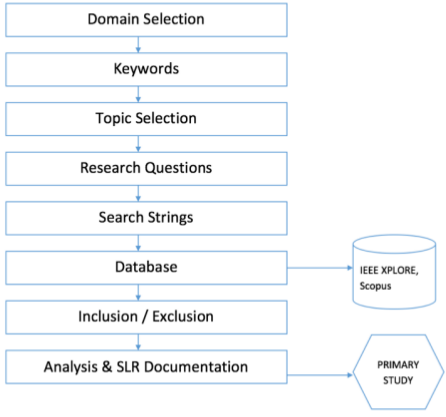
\includegraphics[width=2.5in]{image/process.png}
  \caption{Search process}
  \label{fig:process}
\end{figure}

We finally performed a forward search to get some more results, and found 2 papers this way.
\\
\\
\begin{table}[ht!]
\centering
\addvbuffer[8pt 8pt]{\begin{tabular}{|c|c|c|}
    \hline
    Serial No&Search String&Results\\
    \hline
    1&\makecell{("Optimistic" AND\\ "Contract signing")}&63\\
    \hline
    2&\makecell{("Optimistic" AND\\ "Contract signing"\\ AND "Abuse-free")}&14\\
    \hline
    3&\makecell{Applying inclusion\\ and exclusion criteria}&8\\
    \hline
    4&Forward search&10\\
    \hline
\end{tabular}}
\label{table:ss}
\caption{Search Strings}
\end{table}

